\section{Introduction}
\begin{frame}{\VideoName}
    \tableofcontents[currentsection]
\end{frame}

\begin{frame}{Side-channel attacks}
    \begin{itemize}
        \item Side-channel analysis attacks target cryptographic implementations passively.
       \item The attacks exploit the possibility of the attacker observing the physical characteristics of a device that is running the cryptographic algorithm.
        \item The attacker obtains the side-channel information, e.g. power consumption, and execution time, then utilizes such information to recover the secret key.
     \item  In this course, we will focus on power analysis attacks that exploit power consumption information.
      \item The attack methodologies can be used in a similar manner when electromagnetic emanation (EM) is analyzed.
    \end{itemize}
\begin{alertblock}{Remark}
We use the terminology \textit{side-channel analysis} attacks only in the narrower meaning which refers to power analysis attacks.
In short, we also write side-channel analysis as \textit{SCA}.
\end{alertblock}
\end{frame}

\begin{frame}{Device under test (DUT)}
    \begin{itemize}
        \item The device that we take measurement of is called the \textit{device under test (DUT)}
        \begin{itemize}
            \item a microcontroller running a software implementation
            \item an FPGA or ASIC realizing a hardware implementation.
        \end{itemize}
       \item We assume the attacker has certain knowledge of the implementation.
       \begin{itemize}
           \item how to interface with the encryption routine
           \item whether the computation is executed serially or in parallel
           \item whether some types of countermeasures are present
           \item Generally, this type of information can be also obtained by reverse engineering, visual inspection of the side-channel measurements, or sometimes just with a simple trial-and-error technique.
       \end{itemize}
    \end{itemize}
\end{frame}

\begin{frame}{Attacker goal}
    \begin{itemize}
        \item The ultimate goal of the attacker is to recover the master key of a symmetric block cipher or the private key of a public-key cipher.
    \end{itemize}
\end{frame}

\begin{frame}{Non-profiled SCA}
    \begin{itemize}
        \item If the attacker does not have access to a similar device, just the target device or just the measurements coming from the target device, we talk about \textit{non-profiled SCA}.
        \item In a general scenario, this attack utilizes a set of measurements where a fixed secret key is used to encrypt multiple (random) plaintexts.
    \end{itemize}
\end{frame}

\begin{frame}{Profiled SCA}
    \begin{itemize}
        \item If we assume the attacker has access to a clone device of the target device, then the attacker can carry out a \textit{profiled SCA}.
       \item The attack operates in two phases.
        \item In the profiling phase, the attacker acquires side-channel measurements for known plaintext/ciphertext and known key pairs.
        \begin{itemize}
            \item This set of data is used to characterize or model the device.
        \end{itemize}
        \item Then the attacker acquires a few measurements from the target device, usually identical to the clone device, with known plaintext/ciphertext but the key is secret.
        \begin{itemize}
            \item These measurements from the target device are then tested against the characterized model from the clone device.
        \end{itemize}
    \end{itemize}
\end{frame}

\begin{frame}{Measurement device}
    \begin{itemize}
        \item Power analysis measures the \textit{power consumption} of the device under attack.
        \item The power consumption is in the form of a voltage change.
        \item The measurement is normally done with a digital sampling oscilloscope
         \item We refer to each sample point as a \textit{time sample}.
         % \item An artificial trigger signal that indicates the start/end of the encryption.
    \end{itemize}
\end{frame}

\begin{frame}{Setup}
    \begin{columns}[T] % align columns
\begin{column}{.55\textwidth}
\begin{itemize}
    \item Ready-to-use measurement platform NewAE ChipWhisperer-Lite (black in the middle) -- handling the communication with the DUT and the acquisition.
    \item CW 308 UFO board (red) -- a breakout board with the DUT -- ARM Cortex-M4 (blue) mounted on top.
    \item The controlling and data processing were done from a laptop, from the Jupyter environment available for the ChipWhisperer platform.
    \item Teledyne T3DSO3504 benchtop oscilloscope, used mainly for convenience purposes -- to precisely locate the time intervals in the initial analysis stage.
\end{itemize}
\end{column}%
\hfill%
\begin{column}{.45\textwidth}
\begin{figure}
    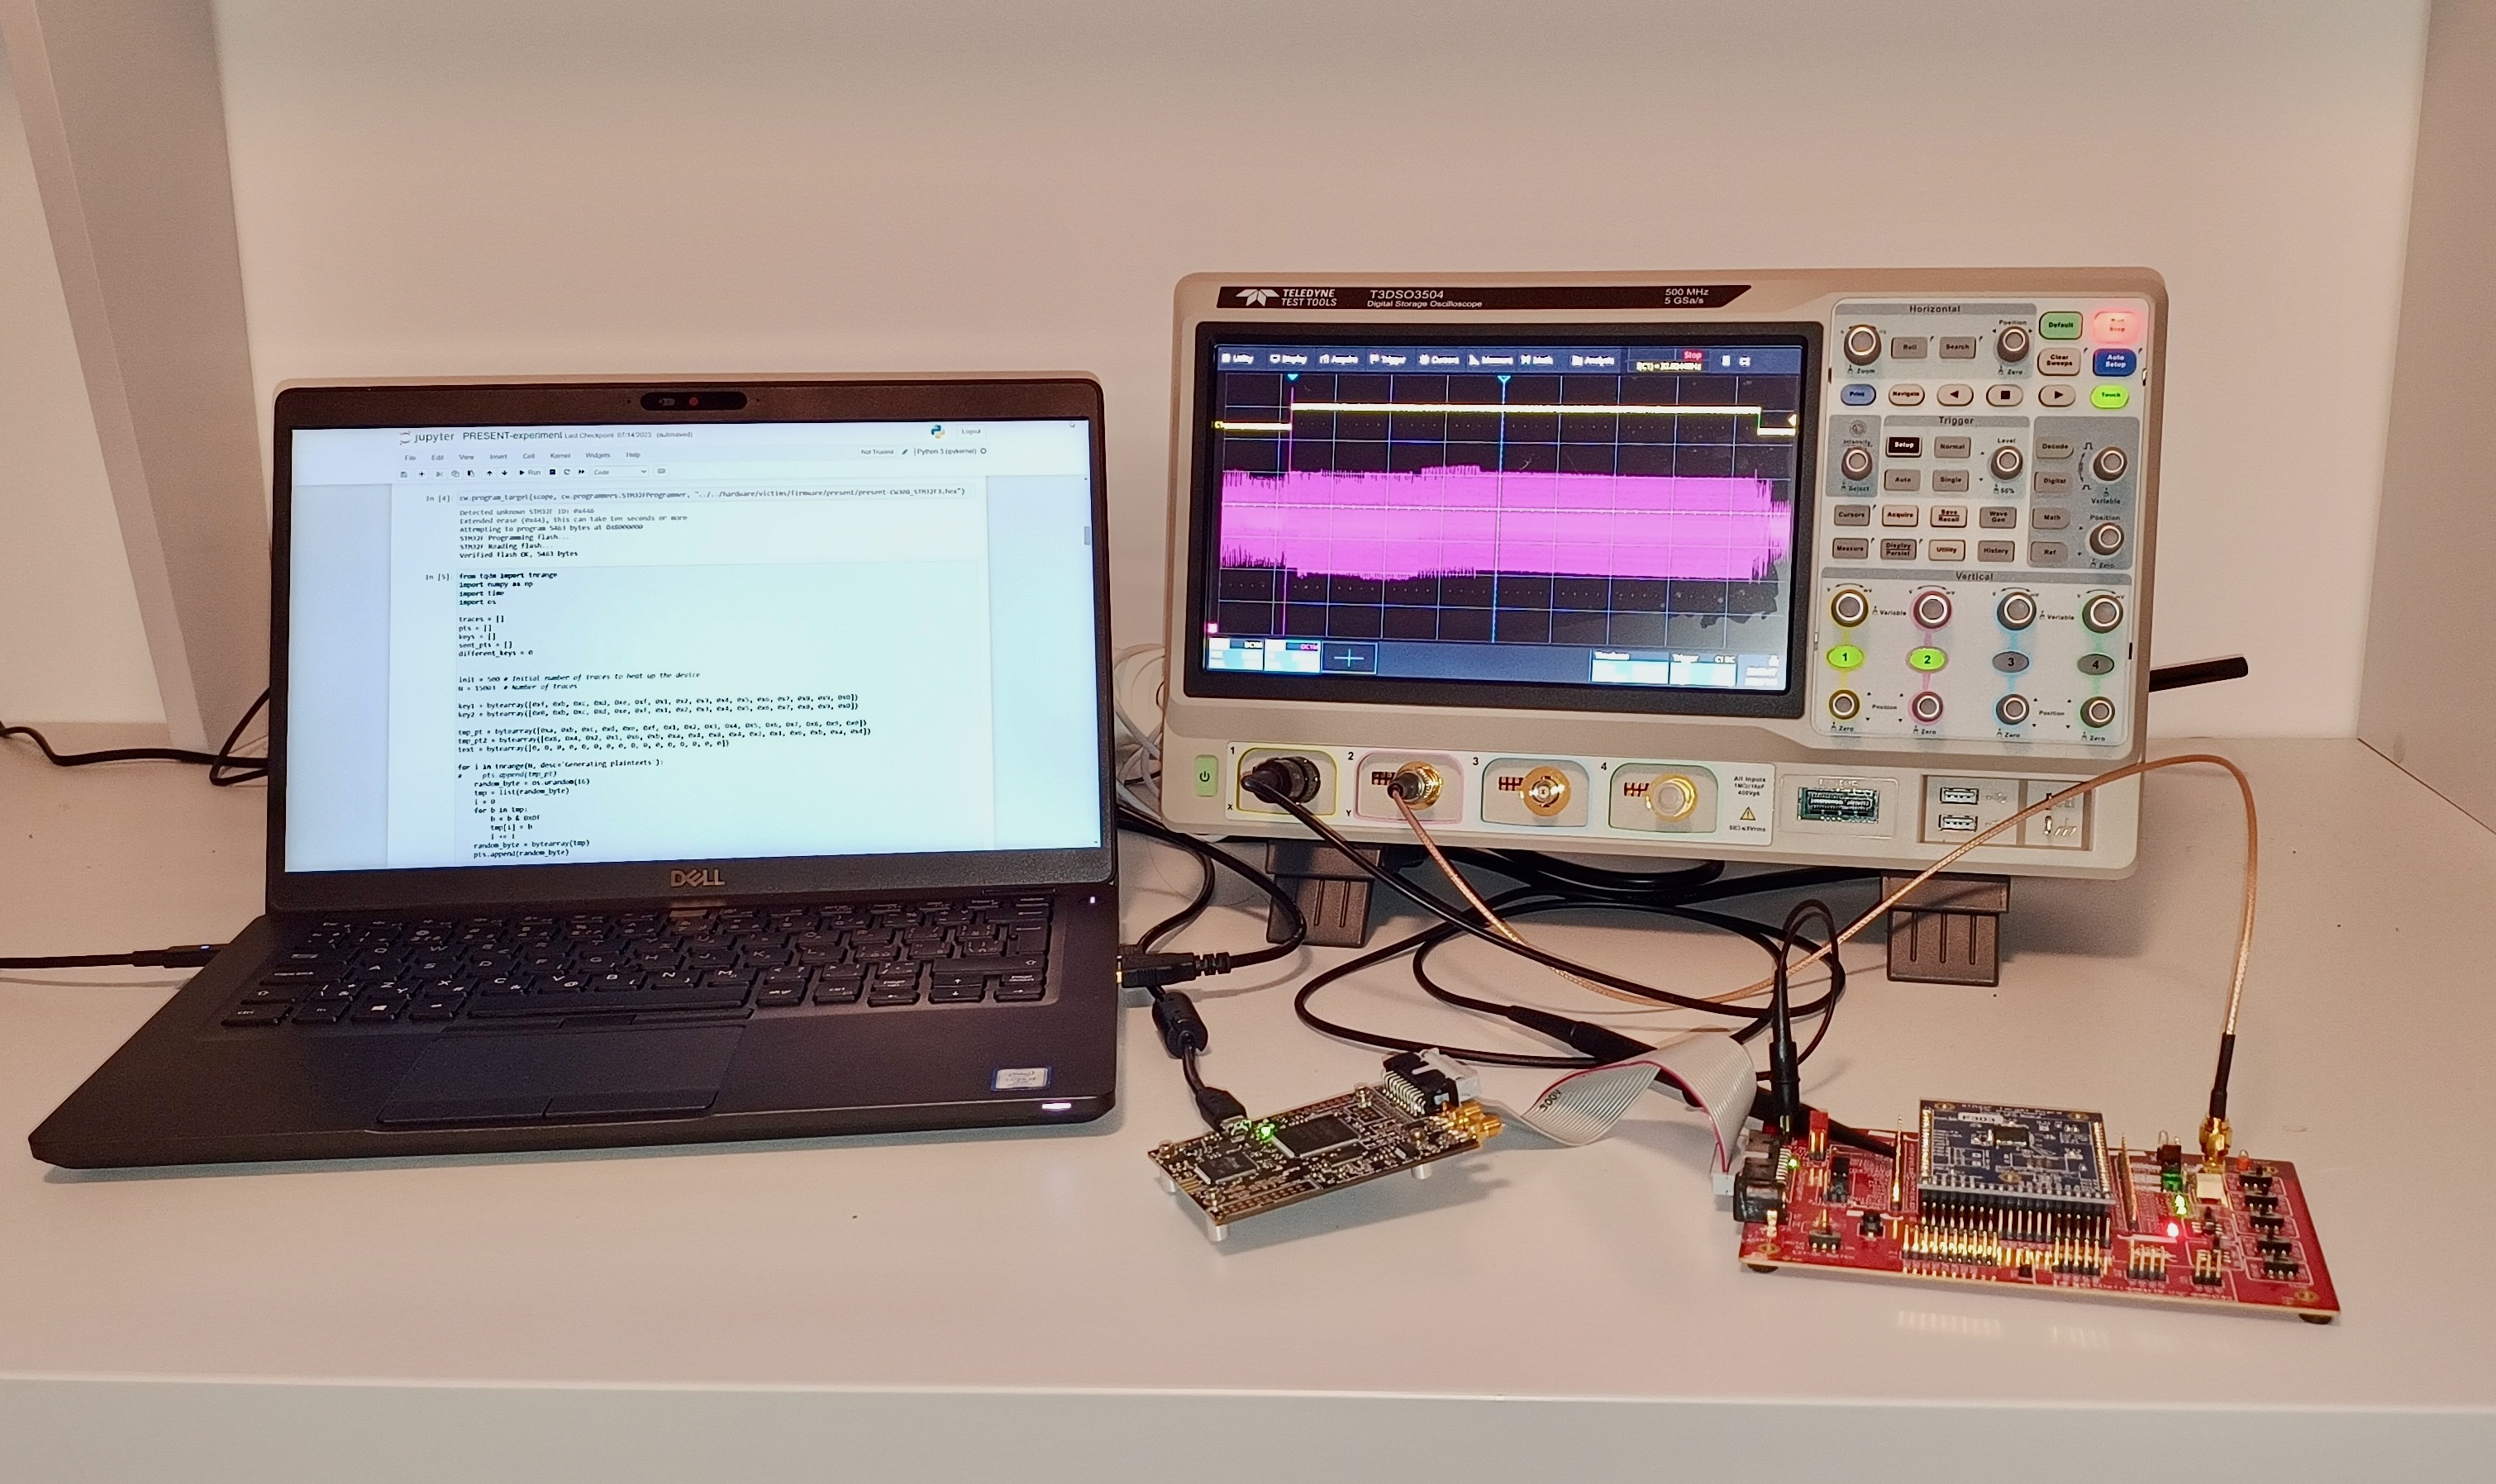
\includegraphics[width=1.1\textwidth]{fig/sca_setup.jpeg}
\end{figure}
\end{column}%
\end{columns}
\end{frame}

\begin{frame}{Experimental setting}
    \begin{itemize}
        \item NewAE ChipWhisperer-Lite. 
       \item The program code was running on a 32-bit ARM Cortex-M4 microcontroller (STM32F3) running with a clock speed of $\approx$ 7.4 MHz.
       \item ADC was set to capture the samples at $4\times$ that speed, i.e. $\approx$ 29.6 MHz
        \item However, for plotting purposes, we normally reduce the number of time samples.
    \end{itemize}
\end{frame}

\begin{frame}{Power trace}
    \begin{itemize}
        \item In our experiments, a trigger signal is raised to high during the computation that we want to capture and lowered afterward.
        \item One measurement consists of the voltage values for each \textit{time sample} in this duration.
        \item It can be stored in an array of length equal to the total number of time samples in the measured time interval.
       \item It can also be drawn in a graph where the $x-$axis corresponds to time samples and the $y-$axis records the voltage values.
       \item Thus, we refer to the result of one measurement as a \textit{(power) trace}.
       \item Note that, in the case of ChipWhisperer, which will be used for our experiments and analysis, the $y-$axis does not show the actual voltage value but a $10$-bit value proportional to the current going through the shunt resistor
    \end{itemize}
\end{frame}



\begin{frame}{One trace}
    \begin{itemize}
        \item One power trace for the first five rounds of PRESENT encryption.
        \item A sequence of \texttt{nop} instructions before and after the cipher computation.
        \item Certain patterns can be seen from the trace and we can deduce the corresponding operations in each time interval.
        \item From time sample $0-312$ and from time sample $2778-3100$ we have \texttt{nop}s.
        \item Five repeated patterns, indicated by red dotted lines $\rightarrow$ duration of each round
    \end{itemize}
    \begin{figure}
        \centering
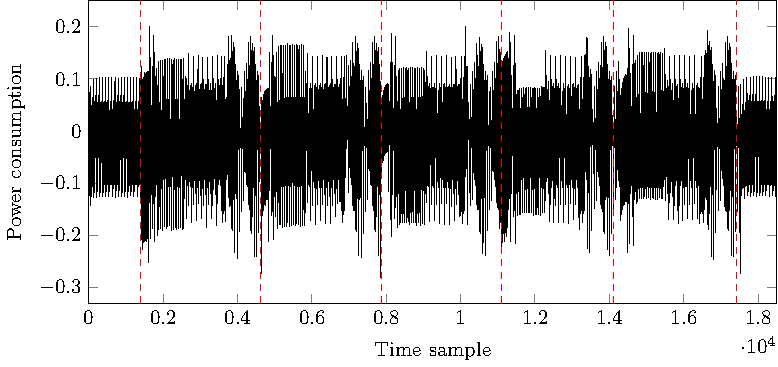
\includegraphics[width=0.7\textwidth]{fig/present_5rounds.pdf}      
    \end{figure}
\end{frame}

\begin{frame}{Datasets}
There are four datasets that will be analyzed in more detail in the course.

All the datasets:
\begin{itemize}
    \item Capture one round of software implementation of PRESENT.
    \item \texttt{nop} instructions before and after PRESENT computation
    \item Each trace has $3600$ time samples
\end{itemize}
More details on individual datasets:
\begin{itemize}
    \item \datafixone: This dataset contains 5000 traces with a fixed round key \texttt{0xFEDCBA0123456789} and a fixed plaintext \texttt{0xABCDEF1234567890}. 
    \item \datafixtwo: This dataset contains 5000 traces with a fixed round key \texttt{0xFEDCBA0123456789} and a fixed plaintext \texttt{0x84216BA484216BA4}.
    \item \dataranone: This dataset contains 5000 traces with a fixed round key \texttt{0xFEDCBA0123456789} and a random plaintext for each trace.
    \item \datarantwo: This dataset contains 10000 traces with a random round key and a random plaintext for each trace.
\end{itemize}
\end{frame}


\begin{frame}{PRESENT -- encryption}
\begin{columns}[T]
\begin{column}{.55\textwidth}
\begin{itemize}
    \item block length: $n=64$
       \item number of rounds: \texttt{Nr}$=31$
       \item key length: either $80$ or $128$.
\end{itemize}
\begin{alertblock}{Remark}
    For PRESENT specification, we consider the $0$th bit of a value as the rightmost bit in its binary representation.
For example, the $0$th bit of $3=011_2$ is $1$, the $1$st bit is $1$ and the $2$nd bit is $0$.
\end{alertblock}
\end{column}%
\hfill%
\begin{column}{.5\textwidth}
\begin{figure}
    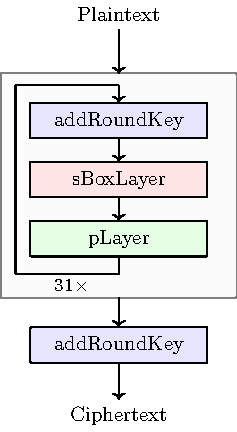
\includegraphics[width=0.6\textwidth]{fig/PRESENT.pdf}
\end{figure}
\end{column}%
\end{columns}
\end{frame}

\begin{frame}{Attack methods}
    \begin{itemize}
        \item Classical power analysis attack methods
        \begin{itemize}
            \item \textit{simple power analysis (SPA)}
            \item \textit{differential power analysis (DPA)}
        \end{itemize}
        \item SPA assumes the attacker has access to only one or a few measurements corresponding to some fixed inputs.
        \item DPA assumes the attacker can take measurements for a potentially unlimited number of different inputs.
    \end{itemize}
\end{frame}

\section{Side-channel Leakages}
\begin{frame}{\VideoName}
    \tableofcontents[currentsection]
\end{frame}

\begin{frame}{Leakages}
    \begin{itemize}
        \item In the later parts of the course, we will see that by analyzing the power consumption, we can deduce the secret key. Consequently, we also refer to the power consumption as the \textit{leakage} of the device.
       \item We consider the leakage consists of two parts: \textit{signal} and \textit{noise}.
       \item Signal refers to the part of the leakage that contains useful information for our attack and the rest is noise.
       \begin{itemize}
           \item For example, if we would like to recover the hamming weight of an intermediate value, then the part of the leakage correlated to the hamming weight of that intermediate value is our signal.
       \end{itemize}
    \end{itemize}
\end{frame}

\begin{frame}{Leakage is dependent on the operations being executed}
    \begin{figure}
    \centering
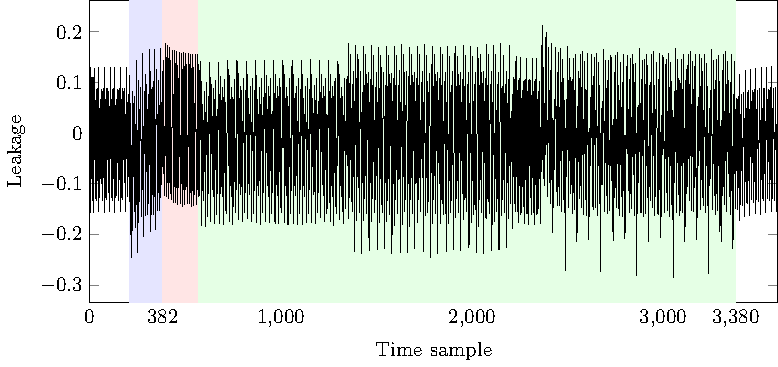
\includegraphics{fig/PRESENT_plot___one_round_average___highlighted_operations.pdf}
    \caption{The averaged trace for $5000$ traces from the \datafixone.
    The blue, pink, and green parts of the trace correspond to addRoundKey, sBoxLayer, and pLayer respectively.}
\end{figure}
\end{frame}

\begin{frame}{Leakage is dependent on the data being processed}
    \begin{itemize}
        \item $1000$ traces: each for a random plaintext with the $0$th bit equal to $0$; Take the average
        \item $1000$ traces: each for a random plaintext with the $0$th bit equal to $1$; Take the average
        \item Take the difference trace of those two averages
    \end{itemize}
\end{frame}

\begin{frame}{Leakage is dependent on the data being processed}
    \begin{itemize}
        \item A few peaks in the difference trace and apart from those peaks, most of the points are close to zero.
       \item Those peaks indicate that at the corresponding time samples, the $0$th bit of the plaintext is involved in the computations.
    \end{itemize}
    \begin{figure}[h]
    \centering
    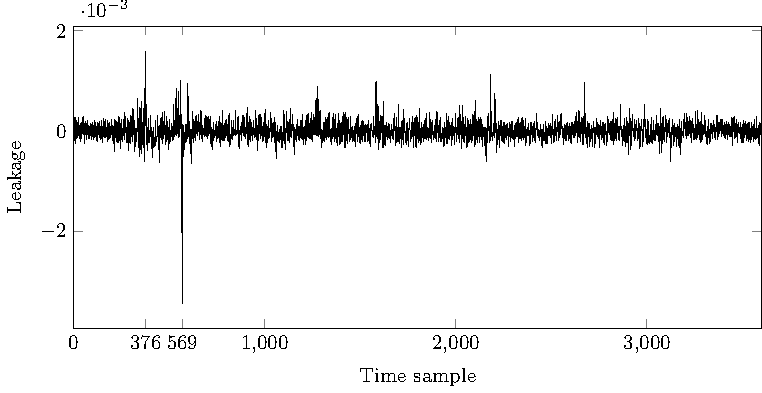
\includegraphics[width=0.8\textwidth]{fig/SCA_PRESENT_bit_dif.pdf}
\end{figure}
\end{frame}

\begin{frame}{Leakage is dependent on the data being processed}
    \begin{itemize}
       \item Compared with the previous figure, we can guess that the first and second peaks most likely correspond to addRoundKey and sBoxLayer.
       \item The later peaks are probably related to the pLayer operation.
    \end{itemize}
    \begin{figure}[h]
    \centering
    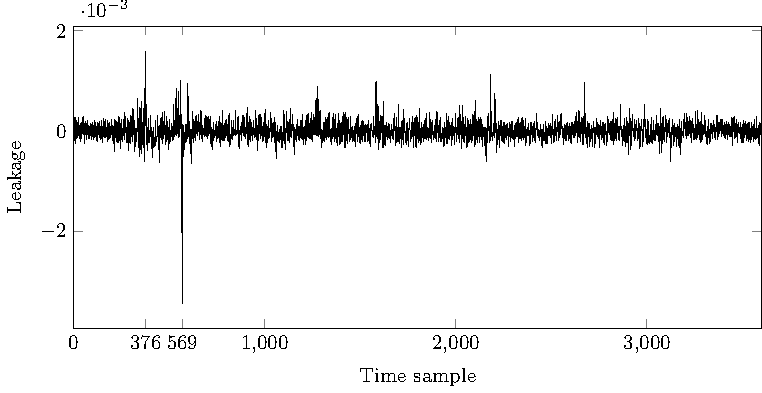
\includegraphics[width=0.8\textwidth]{fig/SCA_PRESENT_bit_dif.pdf}
\end{figure}
\end{frame}

\begin{frame}{Remark}
\begin{itemize}
    \item SPA exploits typically the relationship between the executed operations and the leakage
    \item  DPA focuses on the relationship between the processed data and the leakage
\end{itemize}
\end{frame}

\begin{frame}{Leakage model}
    \begin{itemize}
        \item Assume a value $\boldsymbol{v}$ is being processed in the DUT
        \item Let $\text{noise}\sim\mathcal{N}(0,\sigma^2)$ be a normal random variable with mean $0$ and variance $\sigma^2$.
        \item \textit{identity leakage model}
        \begin{itemize}
            \item the leakage is correlated to $\boldsymbol{v}$
           \[
\mathcal{L}(\boldsymbol{v})=\boldsymbol{v}+\text{noise}.
\]
        \end{itemize}
        \item \textit{Hamming weight model}
        \begin{itemize}
            \item the leakage will then be correlated to $\wt{\boldsymbol{v}}$, the Hamming weight of $\boldsymbol{v}$\footnote{the Hamming weight of vector $\boldsymbol{v}\in\FF_2^m$ is defined to be the number of $1$s in $\boldsymbol{v}$}
            \[
            \mathcal{L}(\boldsymbol{v})=\wt{\boldsymbol{v}}+\text{noise}.
            \]
        \end{itemize}
    \end{itemize}
        \begin{example}
    $\boldsymbol{v}=\texttt{A}$
    \begin{itemize}
        \item identity leakage model: $\mathcal{L}(\boldsymbol{v})=10+\text{noise}$
        \item Hamming weight leakage model: $\mathcal{L}(\boldsymbol{v})=2+\text{noise}$
    \end{itemize}
    \end{example}
\end{frame}

\begin{frame}{Leakage model}
\[
\mathcal{L}(\boldsymbol{v})=\boldsymbol{v}+\text{noise},\quad
  \mathcal{L}(\boldsymbol{v})=\wt{\boldsymbol{v}}+\text{noise}.
\]
    \begin{itemize}
        \item Even though the actual leakage may not be exactly equal to $\mathcal{L}(\boldsymbol{v})$, those leakage models can be used to approximate the behavior of the actual leakages or for statistical analysis.
    \end{itemize}
\end{frame}